% Options for packages loaded elsewhere
\PassOptionsToPackage{unicode}{hyperref}
\PassOptionsToPackage{hyphens}{url}
%
\documentclass[
  letterpaper,
  DIV=11,
  numbers=noendperiod]{scrartcl}

\usepackage{amsmath,amssymb}
\usepackage{iftex}
\ifPDFTeX
  \usepackage[T1]{fontenc}
  \usepackage[utf8]{inputenc}
  \usepackage{textcomp} % provide euro and other symbols
\else % if luatex or xetex
  \usepackage{unicode-math}
  \defaultfontfeatures{Scale=MatchLowercase}
  \defaultfontfeatures[\rmfamily]{Ligatures=TeX,Scale=1}
\fi
\usepackage{lmodern}
\ifPDFTeX\else  
    % xetex/luatex font selection
\fi
% Use upquote if available, for straight quotes in verbatim environments
\IfFileExists{upquote.sty}{\usepackage{upquote}}{}
\IfFileExists{microtype.sty}{% use microtype if available
  \usepackage[]{microtype}
  \UseMicrotypeSet[protrusion]{basicmath} % disable protrusion for tt fonts
}{}
\makeatletter
\@ifundefined{KOMAClassName}{% if non-KOMA class
  \IfFileExists{parskip.sty}{%
    \usepackage{parskip}
  }{% else
    \setlength{\parindent}{0pt}
    \setlength{\parskip}{6pt plus 2pt minus 1pt}}
}{% if KOMA class
  \KOMAoptions{parskip=half}}
\makeatother
\usepackage{xcolor}
\setlength{\emergencystretch}{3em} % prevent overfull lines
\setcounter{secnumdepth}{5}
% Make \paragraph and \subparagraph free-standing
\ifx\paragraph\undefined\else
  \let\oldparagraph\paragraph
  \renewcommand{\paragraph}[1]{\oldparagraph{#1}\mbox{}}
\fi
\ifx\subparagraph\undefined\else
  \let\oldsubparagraph\subparagraph
  \renewcommand{\subparagraph}[1]{\oldsubparagraph{#1}\mbox{}}
\fi


\providecommand{\tightlist}{%
  \setlength{\itemsep}{0pt}\setlength{\parskip}{0pt}}\usepackage{longtable,booktabs,array}
\usepackage{calc} % for calculating minipage widths
% Correct order of tables after \paragraph or \subparagraph
\usepackage{etoolbox}
\makeatletter
\patchcmd\longtable{\par}{\if@noskipsec\mbox{}\fi\par}{}{}
\makeatother
% Allow footnotes in longtable head/foot
\IfFileExists{footnotehyper.sty}{\usepackage{footnotehyper}}{\usepackage{footnote}}
\makesavenoteenv{longtable}
\usepackage{graphicx}
\makeatletter
\def\maxwidth{\ifdim\Gin@nat@width>\linewidth\linewidth\else\Gin@nat@width\fi}
\def\maxheight{\ifdim\Gin@nat@height>\textheight\textheight\else\Gin@nat@height\fi}
\makeatother
% Scale images if necessary, so that they will not overflow the page
% margins by default, and it is still possible to overwrite the defaults
% using explicit options in \includegraphics[width, height, ...]{}
\setkeys{Gin}{width=\maxwidth,height=\maxheight,keepaspectratio}
% Set default figure placement to htbp
\makeatletter
\def\fps@figure{htbp}
\makeatother
% definitions for citeproc citations
\NewDocumentCommand\citeproctext{}{}
\NewDocumentCommand\citeproc{mm}{%
  \begingroup\def\citeproctext{#2}\cite{#1}\endgroup}
\makeatletter
 % allow citations to break across lines
 \let\@cite@ofmt\@firstofone
 % avoid brackets around text for \cite:
 \def\@biblabel#1{}
 \def\@cite#1#2{{#1\if@tempswa , #2\fi}}
\makeatother
\newlength{\cslhangindent}
\setlength{\cslhangindent}{1.5em}
\newlength{\csllabelwidth}
\setlength{\csllabelwidth}{3em}
\newenvironment{CSLReferences}[2] % #1 hanging-indent, #2 entry-spacing
 {\begin{list}{}{%
  \setlength{\itemindent}{0pt}
  \setlength{\leftmargin}{0pt}
  \setlength{\parsep}{0pt}
  % turn on hanging indent if param 1 is 1
  \ifodd #1
   \setlength{\leftmargin}{\cslhangindent}
   \setlength{\itemindent}{-1\cslhangindent}
  \fi
  % set entry spacing
  \setlength{\itemsep}{#2\baselineskip}}}
 {\end{list}}
\usepackage{calc}
\newcommand{\CSLBlock}[1]{\hfill\break\parbox[t]{\linewidth}{\strut\ignorespaces#1\strut}}
\newcommand{\CSLLeftMargin}[1]{\parbox[t]{\csllabelwidth}{\strut#1\strut}}
\newcommand{\CSLRightInline}[1]{\parbox[t]{\linewidth - \csllabelwidth}{\strut#1\strut}}
\newcommand{\CSLIndent}[1]{\hspace{\cslhangindent}#1}

% \usepackage{booktabs}
% \usepackage{soul}
% \usepackage{color}
% \usepackage{amsmath}
% \usepackage{fancyhdr}
% \usepackage{upgreek}
\usepackage{lineno} \linenumbers
\usepackage{setspace} \doublespacing
\usepackage{float}
\usepackage{caption}
\usepackage{subcaption}

\floatplacement{figure}{H}
\floatplacement{table}{H}
\setlength{\parindent}{20pt}

\newcommand{\beginsupplement}{
  \setcounter{table}{0}  
  \renewcommand{\thetable}{S\arabic{table}} 
  \setcounter{figure}{0} 
  \renewcommand{\thefigure}{S\arabic{figure}}
}

\usepackage[many]{tcolorbox}    	% for COLORED BOXES (tikz and xcolor included)
\usepackage{multicol}               % for MULTICOLUMNS

\definecolor{main}{HTML}{5989cf}    % setting main color to be used
\definecolor{sub}{HTML}{cde4ff}     % setting sub color to be used

\usepackage{lscape}
\newcommand{\blandscape}{\begin{landscape}}
\newcommand{\elandscape}{\end{landscape}}

% \tcbset{
%     sharp corners,
%     colback = white,
%     before skip = 0.2cm,    % add extra space before the box
%     after skip = 0.5cm      % add extra space after the box
% }                           % setting global options for tcolorbox

% You can copy any following box you like to your code.
% \newtcolorbox[enhanced,breakable]{boxA}{
%     boxrule = 1.5pt,
%     colframe = black % frame color
% }
\KOMAoption{captions}{tableheading}
\makeatletter
\@ifpackageloaded{caption}{}{\usepackage{caption}}
\AtBeginDocument{%
\ifdefined\contentsname
  \renewcommand*\contentsname{Table of contents}
\else
  \newcommand\contentsname{Table of contents}
\fi
\ifdefined\listfigurename
  \renewcommand*\listfigurename{List of Figures}
\else
  \newcommand\listfigurename{List of Figures}
\fi
\ifdefined\listtablename
  \renewcommand*\listtablename{List of Tables}
\else
  \newcommand\listtablename{List of Tables}
\fi
\ifdefined\figurename
  \renewcommand*\figurename{Figure}
\else
  \newcommand\figurename{Figure}
\fi
\ifdefined\tablename
  \renewcommand*\tablename{Table}
\else
  \newcommand\tablename{Table}
\fi
}
\@ifpackageloaded{float}{}{\usepackage{float}}
\floatstyle{ruled}
\@ifundefined{c@chapter}{\newfloat{codelisting}{h}{lop}}{\newfloat{codelisting}{h}{lop}[chapter]}
\floatname{codelisting}{Listing}
\newcommand*\listoflistings{\listof{codelisting}{List of Listings}}
\makeatother
\makeatletter
\makeatother
\makeatletter
\@ifpackageloaded{caption}{}{\usepackage{caption}}
\@ifpackageloaded{subcaption}{}{\usepackage{subcaption}}
\makeatother
\ifLuaTeX
  \usepackage{selnolig}  % disable illegal ligatures
\fi
\usepackage{bookmark}

\IfFileExists{xurl.sty}{\usepackage{xurl}}{} % add URL line breaks if available
\urlstyle{same} % disable monospaced font for URLs
\hypersetup{
  pdftitle={Environment- and system-specific interactions between traits and population growth},
  hidelinks,
  pdfcreator={LaTeX via pandoc}}

\title{Environment- and system-specific interactions between traits and
population growth}
\author{}
\date{}

\begin{document}
\maketitle
\begin{abstract}
\textbf{Abstract:} Understanding the factors that influence population
dynamics across environmental contexts is essential to predict
ecological stability. Functional traits influence population growth,
which can in turn influence the traits and thus create a feedback
between population and trait dynamics. We analysed the reciprocal
relationship between population and trait dynamics in two microbial
systems (one autotrophic and one heterotrophic system) and across a
range of environmental conditions. When augmenting models of population
(trait) dynamics with trait (population density) data, we found no
consistent improvement of predictive capacity: this improvement was
environment- and system-dependent. Notably, in the cyanobacteria system,
models augmented with population density did predict trait dynamics
better. In addition, when augmented models were superior, the
improvement was substantial. Further investigation of the environmental
dependence of trait-growth relationships is recommended.
\end{abstract}

\newpage{}

\section{Introduction}\label{sec-DAE_introduction}

Forecasting ecological change requires an understanding of population
dynamics, the trajectory of population density through time. A prime
predictor of a population's growth rate is its current density.
Density-dependence of population growth is typically negative,
stimulating growth at low density, while limiting growth at higher
density, which effectively puts a cap on population size. Since the
classic experiments by Gause (\citeproc{ref-Gause1934}{1934}) and Gill
(\citeproc{ref-Gill1972}{1972}), evidence of negative density-dependence
is abundant across biological systems (\citeproc{ref-Sibly2005}{Sibly et
al. 2005}). However, means of functional traits across individuals in a
population have also been proposed as essential predictors of population
growth (\citeproc{ref-Ozgul2012}{Ozgul et al. 2012};
\citeproc{ref-Edwards2013}{Edwards, Litchman, and Klausmeier 2013};
\citeproc{ref-Perez-Ramos2019}{Pérez-Ramos et al. 2019};
\citeproc{ref-Litchman2008}{Litchman and Klausmeier 2008};
\citeproc{ref-Violle2007}{Violle et al. 2007}).

One challenge when using traits to predict population dynamics is that
traits are not static but dynamic. Rapid trait change is widespread
(\citeproc{ref-Ellner2011}{Ellner, Geber, and Hairston 2011}) and, while
trait change caused by environmental change is arguably studied more
often (\citeproc{ref-Grainger2021}{Grainger and Levine 2021}), traits
can also change as a result of population density
(\citeproc{ref-Gibert2022}{Gibert et al. 2022}). This can happen when
population density is strongly-connected to demographic descriptors
(e.g.~size structure \citeproc{ref-Gillooly2001}{Gillooly et al. 2001};
\citeproc{ref-Brown2004}{Brown et al. 2004};
\citeproc{ref-DeLong2015}{DeLong et al. 2015};
\citeproc{ref-Wieczynski2021}{Wieczynski et al. 2021}). In addition, the
trait value itself can be expected to determine trait change, too. This
becomes clear when considering body size, often used as a master trait
predicting population dynamics (\citeproc{ref-Litchman2008}{Litchman and
Klausmeier 2008}). Energetic and physiological costs associated with
body size limit an individual's growth (\citeproc{ref-Frank2009}{Frank
2009}; \citeproc{ref-Schmidt-Nielsen1984}{Schmidt-Nielsen 1984};
\citeproc{ref-Haldane1926}{Haldane 1926}) in much the same way as
population size limits population growth. Two candidate predictors of
trait change therefore stand out: population density and the trait value
itself. Both population growth and trait change therefore represent a
dynamical system of coupled variables. This coupling can create
feedbacks, and is therefore important to unravel if we are to predict
the fate of populations subject to perturbations. One way to formalize
this interdependence of population and trait dynamics is as follows
(\citeproc{ref-Patel2018}{Patel, Cortez, and Schreiber 2018}):

\begin{equation}\phantomsection\label{eq-Patel}{\begin{split}
        \frac{\text{d}N}{N\text{d}t} & = f(N, T) \\
        \frac{\text{d}T}{\text{d}t} & = g(N, T), \\
    \end{split}
}\end{equation}

where \(N\) and \(T\) are the population density and mean trait value
across individuals in a population, and \(f\) and \(g\) are functions
describing the effects of these two predictors on the dynamics of
population density and traits. Note that this framework is general; the
functions \(f\) and \(g\) could capture a variety of biological
mechanisms, including resource competition, and behavioural, epigenetic,
or genetic change. In the context of Equation~\ref{eq-Patel}, the
feedback between population and trait dynamics is captured by the
dependence of \(f\) on \(T\) and of \(g\) on \(N\). If either dependence
is zero, feedback is lost.

Environmental conditions can affect both population growth and
functional traits. For example, in phytoplankton, moderate increases in
temperature increase the growth rate (\citeproc{ref-Brown2004}{Brown et
al. 2004}; \citeproc{ref-Gillooly2001}{Gillooly et al. 2001};
\citeproc{ref-Kremer2017a}{Kremer, Thomas, and Litchman 2017}) while
also favouring smaller cell size
(\citeproc{ref-Fernandez-Gonzalez2021}{Fernández-González and Marañón
2021}). Furthermore, interactions between growth and traits can also be
environment-dependent, as environmental factors such as temperature have
been shown to modulate how traits affect growth
(\citeproc{ref-Brown2004}{Brown et al. 2004};
\citeproc{ref-Gillooly2001}{Gillooly et al. 2001};
\citeproc{ref-Kremer2017a}{Kremer, Thomas, and Litchman 2017}). One may
therefore expect that feedbacks will be environment-dependent, as well
as differing by model systems and which traits are monitored. In systems
where the observed traits have a unequivocal contribution to energy or
resource acquisition, these relationships are expected to be stronger. A
prime example of such systems are primary producers, where traits making
up leaf architecture or pigmentation have a direct link to light and
carbon fixation and therefore fitness and population growth
(\citeproc{ref-Chin2023}{Chin et al. 2023}). In such systems, trait
information may be essential to correctly predict population dynamics
(\citeproc{ref-Stomp2004}{Stomp et al. 2004}) and it is likely that
larger changes to the environment will only increase the importance of
trait information. How the reciprocal effects (of density on traits)
differ between systems is less intuitive, however, and will depend on
the capacity and speed of the trait change.

Here, we investigate the reciprocal links between population and trait
dynamics in two different microbial systems (ciliates and cyanobacteria)
across several environmental conditions. To this end, we performed
microcosm experiments where we monitored population densities and trait
values over time. Given these data, we first asked whether augmenting a
model of density-dependence with traits improved predictions of
population growth. Similarly, we then tested whether augmenting a model
of trait-dependence with population density improved predictions of
trait change. Finally, we asked whether the contributions of traits and
density to population and trait dynamics, respectively, depend on the
environmental context and/or differ between the two model systems.

While we found only limited evidence to support broad feedbacks between
population and trait dynamics, augmenting growth models with trait data
and trait change models with density data often did improve model
performance. These predictive improvements were system- and
environment-specific but were not correlated with the amount of
environmental change. In cases when the augmented model outperformed the
single-state model, the prediction increase was substantial.

\section{Materials and Methods}\label{sec-DAE_methods}

\subsection{Study systems}\label{study-systems}

We addressed these research questions using a number of unicellular,
clonally-reproducing strains from two model systems: seven strains from
four ciliate genera and four strains from two ecotypes of the
picocyanobacteria genus \emph{Synechococcus}
(\citeproc{ref-Farrant2016}{Farrant et al. 2016};
\citeproc{ref-Grebert2018}{Grébert et al. 2018};
\citeproc{ref-Sohm2016}{Sohm et al. 2016}). The ciliate genera are
globally-distributed freshwater mixotrophs and represent an important
ecological link between primary producers and higher trophic levels
(\citeproc{ref-Weisse2022}{Weisse and Montagnes 2022};
\citeproc{ref-Lu2021}{Lu, Gao, and Weisse 2021}). \emph{Synechococcus}
makes up a substantial proportion of marine phytoplankton biomass and
photosynthesis (\citeproc{ref-Dvorak2014}{Dvořák et al. 2014}). Both
study systems harbor considerable diversity, as the freshwater ciliates
span several taxonomic orders and the polyphyetic \emph{Synechoccocus}
has a similar order-level diversity, while, however, being less
well-defined phylogenetically due to the frequency of horizontal gene
transfer events (\citeproc{ref-Salazar2020}{Salazar et al. 2020};
\citeproc{ref-Dvorak2015}{Dvořák et al. 2015};
\citeproc{ref-Zhaxybayeva2006}{Zhaxybayeva et al. 2006}). Both taxa are
commonly-used as model organisms in experiments due to their rapid
growth and relative simplicity. The \emph{Synechococcus} strains used
were purchased from the Roscoff Culture Collection, while the ciliate
strains were isolated from cultures from several collections and
institutions (Section~\ref{sec-culture-origins}).

The ciliate strains selected exhibit substantial diversity in their
functional traits and demography - \emph{Spirostomum} is a large,
elongate, and slow-growing while \emph{Tetrahymena} is small, more
rounded, and faster-growing - and they therefore span a broad range of
ecological niches. Similarly, the \emph{Synechoccocus} strains are
selected from two different ``ecotypes'' that characterise their
pigmentation and biogeography (\citeproc{ref-Stomp2007a}{Stomp et al.
2007}; \citeproc{ref-Sohm2016}{Sohm et al. 2016};
\citeproc{ref-Grebert2018}{Grébert et al. 2018}).

We examined density-dependence and trait-dependence across a range of
environmental conditions, represented here by temperature and a
pollutant --- both commonly-encountered environmental pressures in
natural systems. Specifically, we consider an ``altered'' environment to
have increased temperature, increased concentration of a pollutant, or
both. Both of these pressures are linked to human activity. Temperature
change is ubiquitously-relevant as anthropogenically-driven climate
change continues to intensify. We used atrazine as the pollutant.
Atrazine is present in many aquatic ecosystems via agricultural run-off,
represents a broad class of herbicides that act via the inhibition of
photosynthesis, and also induces oxidative stress in heterotrophic
organisms (e.g.~ciliates), reducing their fitness
(\citeproc{ref-Shim2022}{Shim et al. 2022}). Control conditions are
hereafter indicated by ``C'', temperature changes by ``T'', atrazine
changes by ``A'', and the combined atrazine and temperature changes by
``AT''.

We grew the strain populations in monoculture for sufficient time for
them to reach their carrying capacity, enabling us to track and quantify
their growth and trait changes by measuring the population densities and
trait values at regular, frequent intervals
(Table~\ref{tbl-treatment-table}, Section~\ref{sec-sampling_times}).

\begin{longtable}[]{@{}lllll@{}}
\caption{Experimental design of the two model systems, indicating the
experiment duration, the number of strains used, the temperature of the
warming treatments in degrees Celsius, and the concentration of the
pollutant (atrazine). All combinations of pollution and temperature were
included in the experiment design. Treatments in bold indicate the
reference conditions.}\label{tbl-treatment-table}\tabularnewline
\toprule\noalign{}
Model system & Exp. duration (days) & No.~of strains & Temperature
(\(\mathrm{^\circ C}\)) & Atrazine (\(\mathrm{mg\,L}^{-1}\)) \\
\midrule\noalign{}
\endfirsthead
\toprule\noalign{}
Model system & Exp. duration (days) & No.~of strains & Temperature
(\(\mathrm{^\circ C}\)) & Atrazine (\(\mathrm{mg\,L}^{-1}\)) \\
\midrule\noalign{}
\endhead
\bottomrule\noalign{}
\endlastfoot
Ciliates & \(37\) & \(7\) & \(\mathbf{22}, 24\) & \(\mathbf{0}, 20\) \\
Cyanobacteria & \(10\) & \(4\) & \(\mathbf{22}, 24\) &
\(\mathbf{0}, 0.1\) \\
\end{longtable}

\subsection{Experimental setup}\label{experimental-setup}

For the ciliate system, the microcosms consisted of 250 mL square
bottles with vented caps (DURAN®) containing 100 mL nutrient medium,
inoculated with enough cells to initiate population growth. We obtained
the required cell density by injecting a species-specific volume of
1-week old preculture into new medium (100 \textmu L, 5 mL, 10 mL, and
10 mL for \emph{Tetrahymena thermophila}, \emph{Loxocephalus} sp.,
\emph{Paramecium caudatum} and \emph{Spirostomum teres}, respectively).
The microcosms were kept in an incubator with a 10:14h light/dark cycle.
The nutrient medium consisted of Chalkey's solution supplemented with
crushed protist pellets (Carolina biological supply; 0.55
\(\mathrm{gL}^{-1}\)), filtered through a 0.22 \textmu m filter system
(BT50 500 mL) to remove all particulate matter and consecutively
bacterized with \emph{Bacillus brevis}, \emph{Brevibacillus subtilis}
and \emph{Serratia fonticola}. Following bacterization, the medium was
incubated for two days at 20°C on a shaker to allow the bacteria to grow
before ciliates were added. During the experiment, we replaced 20\% of
the medium every third day by replacing 4 mL culture with 4 mL 5x
concentrated unbacterized nutrient medium, supplemented with atrazine as
needed.

For the cyanobacteria system, the microcosms consisted of 6 mL six-well
plates (Sarstedt standard flat 6 well plate, 83.3920) of PCRS-11 Red Sea
medium (\citeproc{ref-Rippka2000}{Rippka et al. 2000}), inoculated at
5000 cells \(\mathrm{mL}^{-1}\) inside temperature-controlled incubators
(Lovibond Thermostatic Cabinet). They were cultured in white light
(6500K LedAquaristik Sky Bar) in a 12:12h light/dark cycle. The six-well
plates were constantly mixed 150 RPM with a VWR mini shaker.

Growth media were adjusted to include the appropriate amount of atrazine
and microcosms were kept at a constant temperature throughout. All
sampling was undertaken in sterile environments to prevent
contamination.

\subsection{Experimental sampling
procedure}\label{experimental-sampling-procedure}

Population densities and traits were measured using procedures
specifically designed for each species: imaging for ciliates and flow
cytometry for cyanobacteria.

Ciliate microcosms were sampled by digital dark-field imaging using an
much updated version of the method described by Pennekamp and
Schtickzelle (\citeproc{ref-Pennekamp2013}{2013}). For each microcosm,
at each sample time, a series of pictures was taken of a 810 \textmu L
sub-sample using a Sony A9 camera equipped with an FE 90 mm F2.8 Macro G
OSS lens and a dark-field approach (indirect light and black
background). Each series consisted of 10 second burst shots at 10 fps in
grey scale (other settings: 1/160s, F11, ISO 6400), resulting in 100
pictures per sample. We then proceeded with automated image analysis
using Fiji (\citeproc{ref-Schindelin2012}{Schindelin et al. 2012};
\citeproc{ref-VanRossum2022}{Van Rossum 2022}) to count, track, and
characterize the traits of all moving particles i.e.~cell size (area),
cell shape (aspect ratio), movement speed, and movement linearity in the
sample (\citeproc{ref-Pennekamp2014}{Pennekamp et al. 2014}). The traits
were population averages of cell size, cell aspect ratio, linearity of
the cell's movement, and movement speed. Cell morphology influences the
maintenance requirement and resource uptake rates and the motility
traits affect the encounter rate of ciliates for their bacterial
resources.

Cyanobacteria microcosms were sampled using a flow cytometer (Guava
easyCyte 12HT) that measures cell densities and trait values using
several channels, which correspond to specific excitation and
fluorescence combinations by lasers and detectors. The flow cytometer
channels correspond approximately to cell size and concentration of
three photosynthetic pigments present in \emph{Synechococcus}:
chlorophyll-a, phycocyanin, and phycoerythrin. At each sampling time, 57
\textmu  L of distilled water was added to counteract evaporation. Then,
200 \textmu L of the 6 mL microcosm was removed and replaced with 200
\textmu L of fresh medium. This 200 \textmu L sample of the culture was
diluted with distilled water to be between 50 and 500 cells
\textmu \(\mathrm{L}^{-1}\), the concentration range for which the flow
cytometer gives accurate measurements, and 200 \textmu L of the
appropriately-diluted sample was put into a 96-well plate and processed
by the flow cytometer. The flow cytometer then measures 1000 cells from
each well to determine the cell density and measure the trait values.
The traits were population averages of several flow cytometer channels,
indicative of cell size and concentrations of chlorophyll-a,
phycocyanin, \& phycoerythrin. Cell size again influences resource
uptake and maintenance and the photosynthetic pigments influence the
light absorption (\citeproc{ref-Maranon2015}{Marañón 2015};
\citeproc{ref-Stomp2007a}{Stomp et al. 2007}). Sampled debris, dead
cells, and doublets were removed from the analysed data using the
CyanoFilter and PeacoQC packages in R version 2.3.1
(\citeproc{ref-Olusoji2021}{Olusoji et al. 2021};
\citeproc{ref-PeacoQC}{Emmaneel 2022}; \citeproc{ref-RCoreTeam2023}{R
Core Team 2023}).

\subsection{Analyses}\label{analyses}

The objectives of our analyses were to investigate whether we could best
predict the population per-capita growth rate (hereafter ``growth'',
\(\gamma\)) from density only, or if augmenting our prediction using
trait data improved this prediction in our model systems. Similarly, we
tested if augmenting this model using trait data to predict trait change
(hereafter \(\tau\)) with density data improved predictive capacity.

Since there were multiple traits to incorporate, we first summarised the
traits into a single aggregate trait (hereafter ``trait'') using a
principal component analysis, PCA, per strain and treatment. This
eliminates the impact of trait covariance and collinearity, and ensures
that trait information is represented by a single variable, as is
population density. We use only the first component of this PCA to
represent the traits, which contains most of the explained variance
(Figure~\ref{fig-PC-var-explained}, Figure~\ref{fig-PC-var-explained}).

We calculated, for all combinations of strains and environmental
conditions, the growth rate at each time point,
\(\gamma_t=\Delta^{-1}\textrm{log}(N_{t+\Delta}/N_t)\), where \(N\) is
population density and \(\Delta\) is the time between consecutive
sampling times. We then fitted two linear models, for all combinations
of strains and environmental conditions, of \(\gamma_t\) against
\(N_t\):

\begin{equation}\phantomsection\label{eq-pcgr}{
\gamma_t = \beta_0 + \beta_1 N_t,
}\end{equation}

\begin{equation}\phantomsection\label{eq-pcgrExtd}{
\gamma_t = \beta_0 + \beta_1 N_t + \beta_2 T_t,
}\end{equation}

where \(N_t\) (density, continuous) and \(T_t\) (trait value,
continuous) are predictors, and the \(\beta_i\) are regression
coefficients. The first model, Equation~\ref{eq-pcgr}, is the standard
model of linear, density-dependent growth. The second model,
Equation~\ref{eq-pcgrExtd}, is the model augmented with trait data.

Similarly, for all combinations of strains and environmental conditions,
the trait rate of change at each time point \(\tau_t\), as
\(\tau_t=\Delta^{-1}(T_{t+\Delta}-T_{t})\), where \(T\) is the trait
value, and \(\Delta\) is again the time between consecutive sampling
times. We again fitted two models, but now using the trait values as the
response variables:

\begin{equation}\phantomsection\label{eq-dT}{
\tau_t = \beta_0 + \beta_1 T_t,
}\end{equation}

\begin{equation}\phantomsection\label{eq-dTExtd}{
\tau_t = \beta_0 + \beta_1 T_t + \beta_2 N_t,
}\end{equation}

where \(N_t\) (density, continuous) and \(T_t\) (trait value,
continuous) are predictors, and the \(\beta_i\) are regression
coefficients. Again, Equation~\ref{eq-dTExtd} is the augmented version
of Equation~\ref{eq-dT}.

With these models at hand, we then tested whether the augmented model
improved predictions of population/trait dynamics by comparing the
prediction accuracy of the augmented models relative to the basic
models. We compared the AICc (Akaike information criterion corrected for
small sample size \citeproc{ref-Burnham2004}{Burnham and Anderson 2004})
of these models to determine which model best predicted the data,
transforming these AICc values into Akaike scores representing the
probability that the augmented models (Equation~\ref{eq-pcgrExtd},
Equation~\ref{eq-dTExtd}) were better than the basic models
(Equation~\ref{eq-pcgr}, Equation~\ref{eq-dT})
(\citeproc{ref-Wagenmakers2004}{Wagenmakers and Farrell 2004};
\citeproc{ref-Burnham2004}{Burnham and Anderson 2004}). Finally, in
conjunction with the likelihood that the augmented model was best, we
compared the relative change in predictive accuracy, relative to the
single-variable model, using the coefficient of determination
(R-squared).

\section{Results}\label{sec-DAE_results}

\subsection{Observed vs predicted trait and population
change}\label{observed-vs-predicted-trait-and-population-change}

Having fit simple models based on a single variable
(Equation~\ref{eq-pcgr} and Equation~\ref{eq-dT}) as well as the models
augmented using both predictors (Equation~\ref{eq-pcgrExtd} and
Equation~\ref{eq-dTExtd}) on the experimental data
(Figure~\ref{fig-cilia-pcgr} and Figure~\ref{fig-cyano-pcgr}), we first
compare the observed changes in traits and population densities to the
predicted changes using either the single-predictor model or the model
augmented with both predictor variables
(Figure~\ref{fig-growth-dtrait}).

\begin{figure}

\centering{

\includegraphics{figures/growth_dtrait.pdf}

}

\caption{\label{fig-growth-dtrait}Observed (x-axis) and predicted
(y-axis) population growth (top row) and trait change (bottom row),
including either one (left column) or both predictors (right column),
for various strains (point types) of ciliates (left) and cyanobacteria
(right) and across environmental conditions (colours).}

\end{figure}%

\subsection{Model selection}\label{model-selection}

By comparing the Akaike scores of the augmented model we observe that
this model was generally less likely to predict either growth or trait
change for ciliate system across all treatments (Figure~\ref{fig-AIC} a
and c), but was often the better model for the cyanobacteria system
(Figure~\ref{fig-AIC} b and d), particularly for the control and heated
treatments.

\begin{figure}

\centering{

\includegraphics{figures/AIC.pdf}

}

\caption{\label{fig-AIC}Differences in model performance when adding
traits or density to predict growth (top panel) or trait change (bottom
panel) different cilia strains (x-axis) in different treatments
(colour). The mean values across strains and treatments are shown by the
horizontal dashed lines. Values greater than 0.5 indicate that the full
model is likely to be better, values less than 0.5 indicate that the
single-variable model is likely to better, and values around 0.5
indicate that the two models are approximately equal.}

\end{figure}%

In the ciliate system, using the augmented model (including both traits
and population densities) to predict growth/trait change generally did
not improve predictions (Figure~\ref{fig-AIC-deltaerror}). For
predictions of growth, only in a few cases (particularly
\emph{Tetrahymena} strains and \emph{Loxocephalus} 1) was the augmented
model more likely in some environmental conditions. Predictions of trait
change with the augmented model were even less likely to outperform the
trait-only model.

In the cyanobacteria system, for treatments without atrazine, the
augmented models were generally notably better at predicting the system
dynamics (Figure~\ref{fig-AIC}). For predictions of population growth,
the augmented model was generally likely to best describe the data, with
some exceptions in which the added trait data provided no benefit to
predictions. For predictions of trait change, the augmented model was
more likely to be better, with only some cases in the treatments with
atrazine where it failed to improve the predictive ability.

\begin{figure}

\centering{

\includegraphics[width=4in,height=\textheight]{figures/AIC_deltaerror.pdf}

}

\caption{\label{fig-AIC-deltaerror}Comparing the change in predictive
accuracy using the augmented model (both population and traits) as a
response to the probability that the augmented model is best for the
ciliate and cyanobacteria systems. Model accuracy was calculated using
the R-squared statistic.}

\end{figure}%

In the ciliate system, the probability that the augmented model fitted
best was more beneficial when making predictions of population growth
than trait change (Figure~\ref{fig-AIC-deltaerror}). In other words, the
cases in which the augmented model was substantially-better fitting
(e.g.~predictions of growth in \emph{Tetrahymena} 1, control) yielded
more accurate predictions of population growth than trait changes.

In the cyanobacteria system, improvement in predictive accuracy by using
the augmented model was substantial only when the augmented model was
near-certain to be the best (Figure~\ref{fig-AIC-deltaerror}). The
augmented model improved predictions of trait change slightly more than
predictions of population growth.

We do not observe a consistent, cross-system result as to whether
population growth or trait changes are better-predicted by the augmented
model. The relationships are clearly environmentally-dependent and
system-specific, and variation in augmented model performance is
strongly dependent on environmental conditions. That said, for a large
number of the cyanobacteria microcosms, particularly in those without
atrazine added, the augmented model substantially outperforms the
single-variable model (Figure~\ref{fig-AIC-deltaerror}).

\section{Discussion}\label{sec-DAE_discussion}

We have analysed population and trait dynamics in two microbial systems,
across various environmental conditions. Our results do not support a
general reciprocal relationship between both types of dynamics, but do
indicate that trait dynamics are better predicted when considering
population density for the cyanobacteria system, in particular
(Figure~\ref{fig-growth-dtrait}). Furthermore, trait effects on growth
depend on the environment (Figure~\ref{fig-cilia-td-general},
Figure~\ref{fig-cyano-td-general}): a given trait value has differently
effects on growth, depending on the (a)biotic conditions
(\citeproc{ref-Gibert2022}{Gibert et al. 2022};
\citeproc{ref-Wieczynski2021}{Wieczynski et al. 2021}).

Broadly-speaking, the population dynamics of the ciliate system across
most environmental conditions were better-described by simple
density-dependence, as used in most classical population models e.g.
Verhulst (\citeproc{ref-Verhulst1838}{1838}). Density-dependent growth
is clearly a driving force in these cases as the augmented model was not
strongly supported on the basis of Akaike weights (Figure~\ref{fig-AIC})
and the fitted model coefficients were mostly significantly different
from zero (Figure~\ref{fig-cilia-td-general}). Trait dynamics were
similarly generally better-described without including population
density as a covariate (Figure~\ref{fig-AIC}). While intrinsic trait
dynamics are not as well-founded as the equivalent methods in population
dynamics (i.e.~there are no real equivalents of trait intrinsic growth
or carrying capacity), this basic linear trait-dependent trait change
still generally outperformed the augmented model. Trait changes in the
ciliate system, then, seem unlikely to depend on the population density
and, according to these data, feedbacks between populations and traits
in the ciliate system are unlikely.

By contrast, in the cyanobacteria system, the augmented model
outperformed the population-only model in predicting population dynamics
more often than not (Figure~\ref{fig-AIC-deltaerror}) and, in the cases
where it did not fit well, the population-only model was similarly
poorly-fitting (Figure~\ref{fig-R2}). Furthermore, trait dynamics in the
cyanobacteria system were much more consistently well-described by the
augmented model (Figure~\ref{fig-AIC}) and similarly benefitted from the
augmented model in predictive accuracy improvements
(Figure~\ref{fig-AIC-deltaerror}). Particularly in the atrazine-free
treatments, where the augmented model was near-certain to always be
better, but even in the combined atrazine and temperature (AT)
treatments, its performance was overall better. Overall, while
population is only modestly trait-dependent, the trait dynamics are
clearly influenced by population density. In certain cases, therefore,
there is potential for feedbacks between populations and traits
(e.g.~strain V\_2524 in the control and temperature treatments).

There are several possible explanations for the patterns observed.
Firstly, while we assess the linear relationships between traits and
growth rates, it is possible that nonlinear models could more accurately
predict the system dynamics. Nonlinear effects of traits on growth are
commonplace in natural systems (e.g.~the effects of body size on growth
are generally non-linear,
\citeproc{ref-Fernandez-Gonzalez2021}{Fernández-González and Marañón
2021}) and such specifics are lost in the simple model formulation here
although, for the most part, the linear models used seem appropriate
(Figure~\ref{fig-cilia-pcgr}, Figure~\ref{fig-cilia-dT},
Figure~\ref{fig-cyano-pcgr}, Figure~\ref{fig-cyano-dT}).

In a similar manner, the superior performance of the augmented model in
the cyanobacteria system compared to that of the ciliate system may be
due to differences in the traits measured. Firstly that, in the
cyanobacteria system, the aggregate trait summarised more of the trait
information present than in the ciliate system (\(79.5\%\) in the
cyanobacteria system compared to the \(53.6\%\) in the ciliate system,
Figure~\ref{fig-PC-var-explained}). The ciliate traits were more
variable and demonstrated less congruent changes over time
(Figure~\ref{fig-cilia-pop-traits-time}) and it may be that including a
second trait (the second principal component) is a necessary extra
complexity to properly understand population and trait dynamics.
Secondly, it may be that the cyanobacteria traits are more directly
linked to growth than the ciliate traits. For example, the concentration
of photosynthetic pigments within a cell controls absorption of incoming
light and therefore growth. Similarly, the effectiveness of light
harvesting is likely density-dependent (high cell densities cause
shading, which can alter pigmentation), which makes the pigmentation
content subject to plastic change in the time frame of our experiment
(\citeproc{ref-Stomp2004}{Stomp et al. 2004}). Pigmentation and size in
cyanobacteria both constitute resource uptake traits and may both
influence and depend on population growth
(\citeproc{ref-Maranon2015}{Marañón 2015};
\citeproc{ref-Stomp2007a}{Stomp et al. 2007}). In contrast, in the
ciliate system, only one trait, size, could be considered a direct
resource uptake trait. The other ciliate traits (movement linearity,
movement speed, and cell aspect ratio) are less-directly linked to
resource uptake rate and growth. To compute a more directly-functional
aggregate trait for the ciliate system may require a more specific
analysis, for example, by combining the movement and cell size traits
into a clearance rate, which may be more strongly-linked to the growth
of the heterotrophic ciliates (\citeproc{ref-Kiorboe1995}{Kiørboe and
Saiz 1995}; \citeproc{ref-Jacob2019}{Jacob et al. 2019}).

While we summarised the functional traits into a single aggregate trait
per strain and treatment, the individual traits monitored may have
distinct biological responses to the treatments applied and the changes
in population densities. Size changes in response to increased
temperatures is a well-documented phenomenon in microbes
(\citeproc{ref-Finkel2010}{Finkel et al. 2010}). \emph{Synechococcus}
may respond to atrazine exposure by entering a state of chlorosis,
characterised by a loss of chlorophyll and slower growth
(\citeproc{ref-Gonzalez-Barreiro2004}{González-Barreiro et al. 2004}),
although this was not observed in the experimental populations presented
here (Figure~\ref{fig-cyano-pop-traits-time}). Ciliates are known to
adjust their motility and size in response to population density
(\citeproc{ref-Pennekamp2014}{Pennekamp et al. 2014};
\citeproc{ref-Gibert2022}{Gibert et al. 2022}), as shown in
Figure~\ref{fig-cilia-pop-traits-time}.

While we have analysed growth curves and trait dynamics to infer
coupling between density and traits, akin to time series analysis, a
more direct approach would have consisted of a space-for-time approach.
In said approach, one experimentally crosses density and trait values,
and then monitors short-term growth and trait change (e.g.
\citeproc{ref-Wieczynski2021}{Wieczynski et al. 2021}). While
manipulating density is feasible, manipulating traits is less so. One
approach could be to grow cultures at different densities, which we know
will lead to different traits (Figure~\ref{fig-cilia-td-general},
Figure~\ref{fig-cyano-td-general}), and then create density gradients by
dilution. However, such space-for-time approaches do not guarantee a
reliable gradient of functional traits and are more experimentally
demanding.

We find that the potential for feedbacks is limited in our two
experimental systems to a few select cases across the environmental
conditions considered. However, in systems with multiple species present
(i.e.~communities) the potential for feedbacks grows considerably, as
indirect interactions may manifest across multiple species' densities
and traits (e.g. \citeproc{ref-Zelnik2022}{Zelnik et al. 2022}).
However, one challenge will be that the net result of such feedbacks at
the level of population and trait dynamics can be hard to identify, let
alone be predicted.

It is also possible that the trait changes are a result of mutations in
the initially clonal populations. The potential for mutations to take
place during the course of the experiments may differ between the two
model systems due to their population sizes and number of generations
(\citeproc{ref-Barrick2013}{Barrick and Lenski 2013}). Assuming
approximate cell division rates of once per hour and once per day for
the ciliate and cyanobacteria systems, repectively,
(\citeproc{ref-DeLong2009}{DeLong and Hanson 2009};
\citeproc{ref-Binder1995}{Binder and Chisholm 1995}) and accounting for
experiment length (\(\leq 37\) days and \(10\) days), average population
density (\(1.04 \times 10^{3}\) and \(2.23 \times 10^{7}\) cells), and
microcosm volumes (100 mL and 6 mL) gives the number of cell divisions
as \(9.20 \times 10^{7}\) for the ciliate system and
\(1.34 \times 10^{9}\) for the cyanobacteria system. Therefore, we may
expect that the cyanobacteria system possessed somewhat greater
potential for evolution during the course of the experiment, as it is
likely that more cell division events took place. This increased
likelihood of mutation events may have resulted in more prominent
eco-evolutionary dynamics in the cyanobacteria system.

In conclusion, we found that the relationships between populations and
functional traits vary with model system and environmental context.
While reciprocal interactions between density and traits were apparent
for the cyanobacteria system, we did not find broad support for strong
feedbacks between population and trait change. More work is needed to
unveil the context dependence of growth-trait connections.

\subsection{References}\label{references}

\phantomsection\label{refs}
\begin{CSLReferences}{1}{0}
\bibitem[\citeproctext]{ref-Barrick2013}
Barrick, Jeffrey E., and Richard E. Lenski. 2013. {``Genome Dynamics
During Experimental Evolution.''} \emph{Nature Reviews Genetics} 14
(12): 827--39. \url{https://doi.org/10.1038/nrg3564}.

\bibitem[\citeproctext]{ref-Binder1995}
Binder, B J, and S W Chisholm. 1995. {``Cell {Cycle Regulation} in
{Marine Synechococcus} Sp. {Strains}.''} \emph{Applied and Environmental
Microbiology} 61 (2): 708--17.
\url{https://doi.org/10.1128/aem.61.2.708-717.1995}.

\bibitem[\citeproctext]{ref-Brown2004}
Brown, James H., James F. Gillooly, Andrew P. Allen, Van M. Savage, and
Geoffrey B. West. 2004. {``Toward a {Metabolic Theory} of {Ecology}.''}
\emph{Ecology} 85 (7): 1771--89. \url{https://doi.org/10.1890/03-9000}.

\bibitem[\citeproctext]{ref-Burnham2004}
Burnham, Kenneth P., and David R. Anderson. 2004. {``Multimodel
{Inference}: {Understanding AIC} and {BIC} in {Model Selection}.''}
\emph{Sociological Methods \& Research} 33 (2): 261--304.
\url{https://doi.org/10.1177/0049124104268644}.

\bibitem[\citeproctext]{ref-Chin2023}
Chin, Alana R. O., Paula Guzmán-Delgado, Anna Görlich, and Janneke
HilleRisLambers. 2023. {``Towards Multivariate Functional Trait
Syndromes: {Predicting} Foliar Water Uptake in Trees.''} \emph{Ecology},
no. February: 1--15. \url{https://doi.org/10.1002/ecy.4112}.

\bibitem[\citeproctext]{ref-DeLong2015}
DeLong, John P., Benjamin Gilbert, Jonathan B. Shurin, Van M. Savage,
Brandon T. Barton, Christopher F. Clements, Anthony I. Dell, et al.
2015. {``The {Body Size Dependence} of {Trophic Cascades}.''} \emph{The
American Naturalist} 185 (3): 354--66.
\url{https://doi.org/10.1086/679735}.

\bibitem[\citeproctext]{ref-DeLong2009}
DeLong, John P., and David T. Hanson. 2009. {``Metabolic Rate Links
Density to Demography in {Tetrahymena} Pyriformis.''} \emph{The ISME
Journal} 3 (12): 1396--1401.
\url{https://doi.org/10.1038/ismej.2009.81}.

\bibitem[\citeproctext]{ref-Dvorak2014}
Dvořák, Petr, Dale A. Casamatta, Aloisie Poulíčková, Petr Hašler, Vladan
Ondřej, and Remo Sanges. 2014. {``Synechococcus: 3 Billion Years of
Global Dominance.''} \emph{Molecular Ecology} 23 (22): 5538--51.
\url{https://doi.org/10.1111/mec.12948}.

\bibitem[\citeproctext]{ref-Dvorak2015}
Dvořák, Petr, Aloisie Poulíčková, Petr Hašler, Mattia Belli, Dale A.
Casamatta, and Alessio Papini. 2015. {``Species Concepts and Speciation
Factors in Cyanobacteria, with Connection to the Problems of Diversity
and Classification.''} \emph{Biodiversity and Conservation} 24 (4):
739--57. \url{https://doi.org/10.1007/s10531-015-0888-6}.

\bibitem[\citeproctext]{ref-Edwards2013}
Edwards, Kyle F., Elena Litchman, and Christopher A. Klausmeier. 2013.
{``Functional Traits Explain Phytoplankton Responses to Environmental
Gradients Across Lakes of the {United States}.''} \emph{Ecology} 94 (7):
1626--35. \url{https://doi.org/10.1890/12-1459.1}.

\bibitem[\citeproctext]{ref-Ellner2011}
Ellner, Stephen P., Monica A. Geber, and Nelson G. Hairston. 2011.
{``Does Rapid Evolution Matter? {Measuring} the Rate of Contemporary
Evolution and Its Impacts on Ecological Dynamics.''} \emph{Ecology
Letters} 14 (6): 603--14.
\url{https://doi.org/10.1111/j.1461-0248.2011.01616.x}.

\bibitem[\citeproctext]{ref-PeacoQC}
Emmaneel, Annelies. 2022. \emph{{PeacoQC}: {Peak-based} Selection of
High Quality Cytometry Data}. Manual.
\url{https://doi.org/10.18129/B9.bioc.PeacoQC}.

\bibitem[\citeproctext]{ref-Farrant2016}
Farrant, Gregory K., Hugo Doré, Francisco M. Cornejo-Castillo, Frédéric
Partensky, Morgane Ratin, Martin Ostrowski, Frances D. Pitt, et al.
2016. {``Delineating Ecologically Significant Taxonomic Units from
Global Patterns of Marine Picocyanobacteria.''} \emph{Proceedings of the
National Academy of Sciences of the United States of America} 113 (24):
E3365--74. \url{https://doi.org/10.1073/pnas.1524865113}.

\bibitem[\citeproctext]{ref-Fernandez-Gonzalez2021}
Fernández-González, Cristina, and Emilio Marañón. 2021. {``Effect of
Temperature on the Unimodal Size Scaling of Phytoplankton Growth.''}
\emph{Scientific Reports} 11 (1): 953.
\url{https://doi.org/10.1038/s41598-020-79616-0}.

\bibitem[\citeproctext]{ref-Finkel2010}
Finkel, Zoe V., John Beardall, Kevin J. Flynn, Antonietta Quigg, T.
Alwyn V. Rees, and John A. Raven. 2010. {``Phytoplankton in a Changing
World: {Cell} Size and Elemental Stoichiometry.''} \emph{Journal of
Plankton Research} 32 (1): 119--37.
\url{https://doi.org/10.1093/plankt/fbp098}.

\bibitem[\citeproctext]{ref-Frank2009}
Frank, S. A. 2009. {``The Common Patterns of Nature.''} \emph{Journal of
Evolutionary Biology} 22 (8): 1563--85.
\url{https://doi.org/10.1111/j.1420-9101.2009.01775.x}.

\bibitem[\citeproctext]{ref-Gause1934}
Gause, G. F. 1934. {``{EXPERIMENTAL ANALYSIS OF VITO VOLTERRA}'{S
MATHEMATICAL THEORY OF THE STRUGGLE FOR EXISTENCE}.''} \emph{Science
(New York, N.Y.)} 79 (2036): 16--17.
\url{https://doi.org/10.1126/science.79.2036.16-a}.

\bibitem[\citeproctext]{ref-Gibert2022}
Gibert, Jean P., Ze-Yi Han, Daniel J. Wieczynski, Samantha Votzke, and
Andrea Yammine. 2022. {``Feedbacks Between Size and Density Determine
Rapid Eco-Phenotypic Dynamics.''} \emph{Functional Ecology} 36 (7):
1668--80. \url{https://doi.org/10.1111/1365-2435.14070}.

\bibitem[\citeproctext]{ref-Gill1972}
Gill, Doublas E. 1972. {``Density {Dependence} and {Population
Regulation} in {Laboratory Cultures} of {Paramecium}.''} \emph{Ecology}
53 (4): 701--8. \url{https://doi.org/10.2307/1934786}.

\bibitem[\citeproctext]{ref-Gillooly2001}
Gillooly, James F., James H. Brown, Geoffrey B. West, Van M. Savage, and
Eric L. Charnov. 2001. {``Effects of {Size} and {Temperature} on
{Metabolic Rate}.''} \emph{Science} 293 (5538): 2248--51.
\url{https://doi.org/10.1126/science.1061967}.

\bibitem[\citeproctext]{ref-Gonzalez-Barreiro2004}
González-Barreiro, Óscar, Carmen Rioboo, Angeles Cid, and Concepción
Herrero. 2004. {``Atrazine-{Induced Chlorosis} in {Synechococcus}
Elongatus {Cells}.''} \emph{Archives of Environmental Contamination and
Toxicology} 46 (3): 301--7.
\url{https://doi.org/10.1007/s00244-003-2149-z}.

\bibitem[\citeproctext]{ref-Grainger2021}
Grainger, Tess Nahanni, and Jonathan M. Levine. 2021. {``Rapid Evolution
of Life-History Traits in Response to Warming, Predation and
Competition: {A} Meta-Analysis.''} \emph{Ecology Letters} n/a (n/a).
\url{https://doi.org/10.1111/ele.13934}.

\bibitem[\citeproctext]{ref-Grebert2018}
Grébert, Théophile, Hugo Doré, Frédéric Partensky, Gregory K. Farrant,
Emmanuel S. Boss, Marc Picheral, Lionel Guidi, et al. 2018. {``Light
Color Acclimation Is a Key Process in the Global Ocean Distribution of
{Synechococcus} Cyanobacteria.''} \emph{Proceedings of the National
Academy of Sciences of the United States of America} 115 (9): E2010--19.
\url{https://doi.org/10.1073/pnas.1717069115}.

\bibitem[\citeproctext]{ref-Haldane1926}
Haldane, John BS. 1926. {``On Being the Right Size.''} \emph{Harper's
Magazine} 152: 424--27.

\bibitem[\citeproctext]{ref-Jacob2019}
Jacob, Staffan, Alexis S. Chaine, Michèle Huet, Jean Clobert, and
Delphine Legrand. 2019. {``Variability in Dispersal Syndromes Is a Key
Driver of Metapopulation Dynamics in Experimental Microcosms.''}
\emph{American Naturalist} 194 (5): 613--26.
\url{https://doi.org/10.1086/705410}.

\bibitem[\citeproctext]{ref-Kiorboe1995}
Kiørboe, Thomas, and Enric Saiz. 1995. {``Planktivorous Feeding in Calm
and Turbulent Environments, with Emphasis on Copepods.''} \emph{Marine
Ecology Progress Series} 122 (1/3): 135--45.
\url{https://www.jstor.org/stable/24852263}.

\bibitem[\citeproctext]{ref-Kremer2017a}
Kremer, Colin T., Mridul K. Thomas, and Elena Litchman. 2017.
{``Temperature- and Size-Scaling of Phytoplankton Population Growth
Rates: {Reconciling} the {Eppley} Curve and the Metabolic Theory of
Ecology.''} \emph{Limnology and Oceanography} 62 (4): 1658--70.
\url{https://doi.org/10.1002/lno.10523}.

\bibitem[\citeproctext]{ref-Litchman2008}
Litchman, Elena, and Christopher A. Klausmeier. 2008. {``Trait-{Based
Community Ecology} of {Phytoplankton}.''} \emph{Annual Review of
Ecology, Evolution, and Systematics} 39 (1): 615--39.
\url{https://doi.org/10.1146/annurev.ecolsys.39.110707.173549}.

\bibitem[\citeproctext]{ref-Lu2021}
Lu, Xiaoteng, Yunyi Gao, and Thomas Weisse. 2021. {``Functional Ecology
of Two Contrasting Freshwater Ciliated Protists in Relation to
Temperature.''} \emph{Journal of Eukaryotic Microbiology} 68 (1): 1--16.
\url{https://doi.org/10.1111/jeu.12823}.

\bibitem[\citeproctext]{ref-Maranon2015}
Marañón, Emilio. 2015. {``Cell {Size} as a {Key Determinant} of
{Phytoplankton Metabolism} and {Community Structure}.''} \emph{Annual
Review of Marine Science} 7 (1): 241--64.
\url{https://doi.org/10.1146/annurev-marine-010814-015955}.

\bibitem[\citeproctext]{ref-Olusoji2021}
Olusoji, Oluwafemi D., Jurg W. Spaak, Mark Holmes, Thomas Neyens, Marc
Aerts, and Frederik De Laender. 2021. {``{cyanoFilter}: {An R} Package
to Identify Phytoplankton Populations from Flow Cytometry Data Using
Cell Pigmentation and Granularity.''} \emph{Ecological Modelling} 460
(November): 109743.
\url{https://doi.org/10.1016/j.ecolmodel.2021.109743}.

\bibitem[\citeproctext]{ref-Ozgul2012}
Ozgul, Arpat, Tim Coulson, Alan Reynolds, Tom C. Cameron, and Tim G.
Benton. 2012. {``Population Responses to Perturbations: {The} Importance
of Trait-Based Analysis Illustrated Through a Microcosm Experiment.''}
\emph{American Naturalist} 179 (5): 582--94.
\url{https://doi.org/10.1086/664999}.

\bibitem[\citeproctext]{ref-Patel2018}
Patel, Swati, Michael H. Cortez, and Sebastian J. Schreiber. 2018.
{``Partitioning the {Effects} of {Eco-Evolutionary Feedbacks} on
{Community Stability}.''} \emph{The American Naturalist} 191 (3):
381--94. \url{https://doi.org/10.1086/695834}.

\bibitem[\citeproctext]{ref-Pennekamp2014}
Pennekamp, Frank, Katherine A. Mitchell, Alexis Chaine, and Nicolas
Schtickzelle. 2014. {``Dispersal {Propensity} in {Tetrahymena}
Thermophila {Ciliates} - a {Reaction Norm Perspective}.''}
\emph{Evolution; International Journal of Organic Evolution} 68 (8):
2319--30. \url{https://doi.org/10.1111/evo.12428}.

\bibitem[\citeproctext]{ref-Pennekamp2013}
Pennekamp, Frank, and Nicolas Schtickzelle. 2013. {``Implementing Image
Analysis in Laboratory-Based Experimental Systems for Ecology and
Evolution: {A} Hands-on Guide.''} \emph{Methods in Ecology and
Evolution} 4 (5): 483--92.
\url{https://doi.org/10.1111/2041-210X.12036}.

\bibitem[\citeproctext]{ref-Perez-Ramos2019}
Pérez-Ramos, Ignacio M., Luis Matías, Lorena Gómez-Aparicio, and Óscar
Godoy. 2019. {``Functional Traits and Phenotypic Plasticity Modulate
Species Coexistence Across Contrasting Climatic Conditions.''}
\emph{Nature Communications} 10 (1): 2555.
\url{https://doi.org/10.1038/s41467-019-10453-0}.

\bibitem[\citeproctext]{ref-RCoreTeam2023}
R Core Team. 2023. \emph{R: {A} Language and Environment for Statistical
Computing}. Manual. {Vienna, Austria}: {R Foundation for Statistical
Computing}.

\bibitem[\citeproctext]{ref-Rippka2000}
Rippka, R., T. Coursin, W. Hess, C. Lichtle, D. J. Scanlan, K. A.
Palinska, I. Iteman, F. Partensky, J. Houmard, and M. Herdman. 2000.
{``Prochlorococcus Marinus {Chisholm} Et Al. 1992 Subsp. Pastoris Subsp.
Nov. Strain {PCC} 9511, the First Axenic Chlorophyll A2/B2-Containing
Cyanobacterium ({Oxyphotobacteria}).''} \emph{International Journal of
Systematic and Evolutionary Microbiology} 50 (5): 1833--47.
\url{https://doi.org/10.1099/00207713-50-5-1833}.

\bibitem[\citeproctext]{ref-Salazar2020}
Salazar, Vinícius W., Diogo A. Tschoeke, Jean Swings, Carlos A. Cosenza,
Marta Mattoso, Cristiane C. Thompson, and Fabiano L. Thompson. 2020.
{``A New Genomic Taxonomy System for the {Synechococcus} Collective.''}
\emph{Environmental Microbiology} 22 (11): 4557--70.
\url{https://doi.org/10.1111/1462-2920.15173}.

\bibitem[\citeproctext]{ref-Schindelin2012}
Schindelin, Johannes, Ignacio Arganda-Carreras, Erwin Frise, Verena
Kaynig, Mark Longair, Tobias Pietzsch, Stephan Preibisch, et al. 2012.
{``Fiji: {An} Open-Source Platform for Biological-Image Analysis.''}
\emph{Nature Methods} 9 (7): 676--82.
\url{https://doi.org/10.1038/nmeth.2019}.

\bibitem[\citeproctext]{ref-Schmidt-Nielsen1984}
Schmidt-Nielsen, Knut. 1984. \emph{Scaling: {Why} Is {Animal Size So
Important}?} {Cambridge University Press}.

\bibitem[\citeproctext]{ref-Shim2022}
Shim, Kyu Young, Vrinda Sukumaran, In Cheol Yeo, Heesang Shin, and Chang
Bum Jeong. 2022. {``Effects of Atrazine and Diuron on Life Parameters,
Antioxidant Response, and Multixenobiotic Resistance in Non-Targeted
Marine Zooplankton.''} \emph{Comparative Biochemistry and Physiology
Part - C: Toxicology and Pharmacology} 258 (May): 109378.
\url{https://doi.org/10.1016/j.cbpc.2022.109378}.

\bibitem[\citeproctext]{ref-Sibly2005}
Sibly, Richard M., Daniel Barker, Michael C. Denham, Jim Hone, and Mark
Pagel. 2005. {``On the {Regulation} of {Populations} of {Mammals},
{Birds}, {Fish}, and {Insects}.''} \emph{Science} 309 (5734): 607--10.
\url{https://doi.org/10.1126/science.1110760}.

\bibitem[\citeproctext]{ref-Sohm2016}
Sohm, Jill A., Nathan A. Ahlgren, Zachary J. Thomson, Cheryl Williams,
James W. Moffett, Mak A. Saito, Eric A. Webb, and Gabrielle Rocap. 2016.
{``Co-Occurring {Synechococcus} Ecotypes Occupy Four Major Oceanic
Regimes Defined by Temperature, Macronutrients and Iron.''} \emph{ISME
Journal} 10 (2): 333--45. \url{https://doi.org/10.1038/ismej.2015.115}.

\bibitem[\citeproctext]{ref-Stomp2004}
Stomp, Maayke, Jef Huisman, Floris De Jongh, Annelies J. Veraart, Daan
Gerla, Machteld Rijkeboer, Bas W. Ibelings, Ute I. A. Wollenzien, and
Lucas J. Stal. 2004. {``Adaptive Divergence in Pigment Composition
Promotes Phytoplankton Biodiversity.''} \emph{Nature} 432 (7013):
104--7. \url{https://doi.org/10.1038/nature03044}.

\bibitem[\citeproctext]{ref-Stomp2007a}
Stomp, Maayke, Jef Huisman, Lucas J. Stal, and Hans C. P. Matthijs.
2007. {``Colorful Niches of Phototrophic Microorganisms Shaped by
Vibrations of the Water Molecule.''} \emph{ISME Journal} 1 (4): 271--82.
\url{https://doi.org/10.1038/ismej.2007.59}.

\bibitem[\citeproctext]{ref-VanRossum2022}
Van Rossum, G. 2022. {``The Python Language Reference: {Expressions}.''}
\emph{Python Reference Manual}, 11.

\bibitem[\citeproctext]{ref-Verhulst1838}
Verhulst, Pierre-François. 1838. {``Notice Sur La Loi Que La Population
Suit Dans Son Accroissement.''} \emph{Correspondence Mathematique Et
Physique} 10: 113--29.

\bibitem[\citeproctext]{ref-Violle2007}
Violle, Cyrille, Marie-Laure Navas, Denis Vile, Elena Kazakou, Claire
Fortunel, Irène Hummel, and Eric Garnier. 2007. {``Let the Concept of
Trait Be Functional!''} \emph{Oikos} 116 (5): 882--92.
\url{https://doi.org/10.1111/j.0030-1299.2007.15559.x}.

\bibitem[\citeproctext]{ref-Wagenmakers2004}
Wagenmakers, Eric-Jan, and Simon Farrell. 2004. {``{AIC} Model Selection
Using {Akaike} Weights.''} \emph{Psychonomic Bulletin \& Review} 11 (1):
192--96. \url{https://doi.org/10.3758/BF03206482}.

\bibitem[\citeproctext]{ref-Weisse2022}
Weisse, Thomas, and David J. S. Montagnes. 2022. {``Ecology of
Planktonic Ciliates in a Changing World: {Concepts}, Methods, and
Challenges.''} \emph{Journal of Eukaryotic Microbiology} 69 (5): 1--16.
\url{https://doi.org/10.1111/jeu.12879}.

\bibitem[\citeproctext]{ref-Wieczynski2021}
Wieczynski, Daniel J., Pranav Singla, Adrian Doan, Alexandra Singleton,
Ze-Yi Han, Samantha Votzke, Andrea Yammine, and Jean P. Gibert. 2021.
{``Linking Species Traits and Demography to Explain Complex Temperature
Responses Across Levels of Organization.''} \emph{Proceedings of the
National Academy of Sciences} 118 (42).
\url{https://doi.org/10.1073/pnas.2104863118}.

\bibitem[\citeproctext]{ref-Zelnik2022}
Zelnik, Yuval R., Nuria Galiana, Matthieu Barbier, Michel Loreau, Eric
Galbraith, and Jean-François Arnoldi. 2022. {``How Collectively
Integrated Are Ecological Communities?''} Preprint. {Ecology}.
\url{https://doi.org/10.1101/2022.12.29.522189}.

\bibitem[\citeproctext]{ref-Zhaxybayeva2006}
Zhaxybayeva, Olga, J. Peter Gogarten, Robert L. Charlebois, W. Ford
Doolittle, and R. Thane Papke. 2006. {``Phylogenetic Analyses of
Cyanobacterial Genomes: {Quantification} of Horizontal Gene Transfer
Events.''} \emph{Genome Research} 16 (9): 1099--1108.
\url{https://doi.org/10.1101/gr.5322306}.

\end{CSLReferences}

\newpage{}

\beginsupplement

\section{Supplementary}\label{supplementary}

\singlespacing

\section{Culture origins}\label{sec-culture-origins}

The ciliate strains were isolated from cultures used for past
experiments.

\begin{longtable}[]{@{}
  >{\raggedright\arraybackslash}p{(\columnwidth - 6\tabcolsep) * \real{0.1268}}
  >{\raggedright\arraybackslash}p{(\columnwidth - 6\tabcolsep) * \real{0.3803}}
  >{\raggedright\arraybackslash}p{(\columnwidth - 6\tabcolsep) * \real{0.2676}}
  >{\raggedright\arraybackslash}p{(\columnwidth - 6\tabcolsep) * \real{0.2254}}@{}}
\toprule\noalign{}
\begin{minipage}[b]{\linewidth}\raggedright
\textbf{Name}
\end{minipage} & \begin{minipage}[b]{\linewidth}\raggedright
\textbf{Strain}
\end{minipage} & \begin{minipage}[b]{\linewidth}\raggedright
\textbf{Origin}
\end{minipage} & \begin{minipage}[b]{\linewidth}\raggedright
\end{minipage} \\
\midrule\noalign{}
\endhead
\bottomrule\noalign{}
\endlastfoot
Tetra\_1 & \emph{Tetrahymena} TSC SD01546 & American Type Center
Collection & \\
Tetra\_2 & \emph{Tetrahymena} TSC SD01548 & American Type Center
Collection & \\
Loxo\_1 & \emph{Loxocephalus} & Carolina Biological Supplies & \\
Loxo\_2 & \emph{Loxocephalus} & Carolina Biological Supplies & \\
Para\_4 & \emph{Paramecium} & Carolina Biological Supplies & \\
Spiro\_C & \emph{Spirostomum} & & \\
Spiro\_D & \emph{Spirostomum} & & \\
\end{longtable}

The cyanobacteria strains were purchased from the Roscoff Culture
Collection (\url{https://roscoff-culture-collection.org/}) and they are
referred to throughout using their RCC Number.

\begin{longtable}[]{@{}
  >{\raggedright\arraybackslash}p{(\columnwidth - 8\tabcolsep) * \real{0.2778}}
  >{\raggedright\arraybackslash}p{(\columnwidth - 8\tabcolsep) * \real{0.1806}}
  >{\raggedright\arraybackslash}p{(\columnwidth - 8\tabcolsep) * \real{0.1806}}
  >{\raggedright\arraybackslash}p{(\columnwidth - 8\tabcolsep) * \real{0.1806}}
  >{\raggedright\arraybackslash}p{(\columnwidth - 8\tabcolsep) * \real{0.1806}}@{}}
\toprule\noalign{}
\begin{minipage}[b]{\linewidth}\raggedright
\textbf{Name / RCC number}
\end{minipage} & \begin{minipage}[b]{\linewidth}\raggedright
\textbf{Strain}
\end{minipage} & \begin{minipage}[b]{\linewidth}\raggedright
\textbf{\emph{Synechococcus}} \textbf{clade}
\end{minipage} & \begin{minipage}[b]{\linewidth}\raggedright
\textbf{Pigment type}
\end{minipage} & \begin{minipage}[b]{\linewidth}\raggedright
\textbf{Isolation}
\end{minipage} \\
\midrule\noalign{}
\endhead
\bottomrule\noalign{}
\endlastfoot
2375 & BL\_10 & Subcluster 5.1 V & 2 & W. Sahara \\
2434 & RS9906 & Subcluster 5.1 VIII & 1 & Israel \\
2524 & A15-46 & Subcluster 5.1 V & 2 & Spain \\
2383 & RS9909 & Subcluster 5.1 VIII & 1 & Israel \\
\end{longtable}

\section{Sampling regime}\label{sec-sampling_times}

\subsection{Ciliate}\label{ciliate}

Due to the large differences in cilate population dynamics, the sampling
differed between species. Furthermore, since the most important
information required to fit growth curves was towards the start of the
experiment (in the exponential growth phase), sampling was more frequent
at the beginning of the experiment and then declined in frequency as the
populations stabilised. \emph{Tetrahhymena} strains were sampled twice a
day during the first week at 09:00 and 17:00. All other species were
sampled once a day during the first week at 13:00. During the second
week, all species were sample once a day at 13:00. During the third
week, all species were sampled every second day at 13:00. Finally,
during the fourth and fifth weeks, all species were sampled twice a week
on Mondays and Thursdays at 13:00.

\subsection{Cyanobacteria}\label{cyanobacteria}

The cyanobacteria microcosms were sampled every day at the same time for
each microcosm: between 09:00 and 13:00 depending on the population, as
the sampling procedure took some time. Additionally, each microcosm of
the cyanobacteria system had three replicates.

\subsection{Growth and trait change}\label{growth-and-trait-change}

The ciliate populations grew logistically in all conditions, approaching
a roughly stable state by the end of the experiment
(Figure~\ref{fig-cilia-pop-traits-time}). The final population densities
differed greatly between genera, with \emph{Tetrahymena} reaching
densities an order of magnitude greater than the others.

\begin{figure}

\centering{

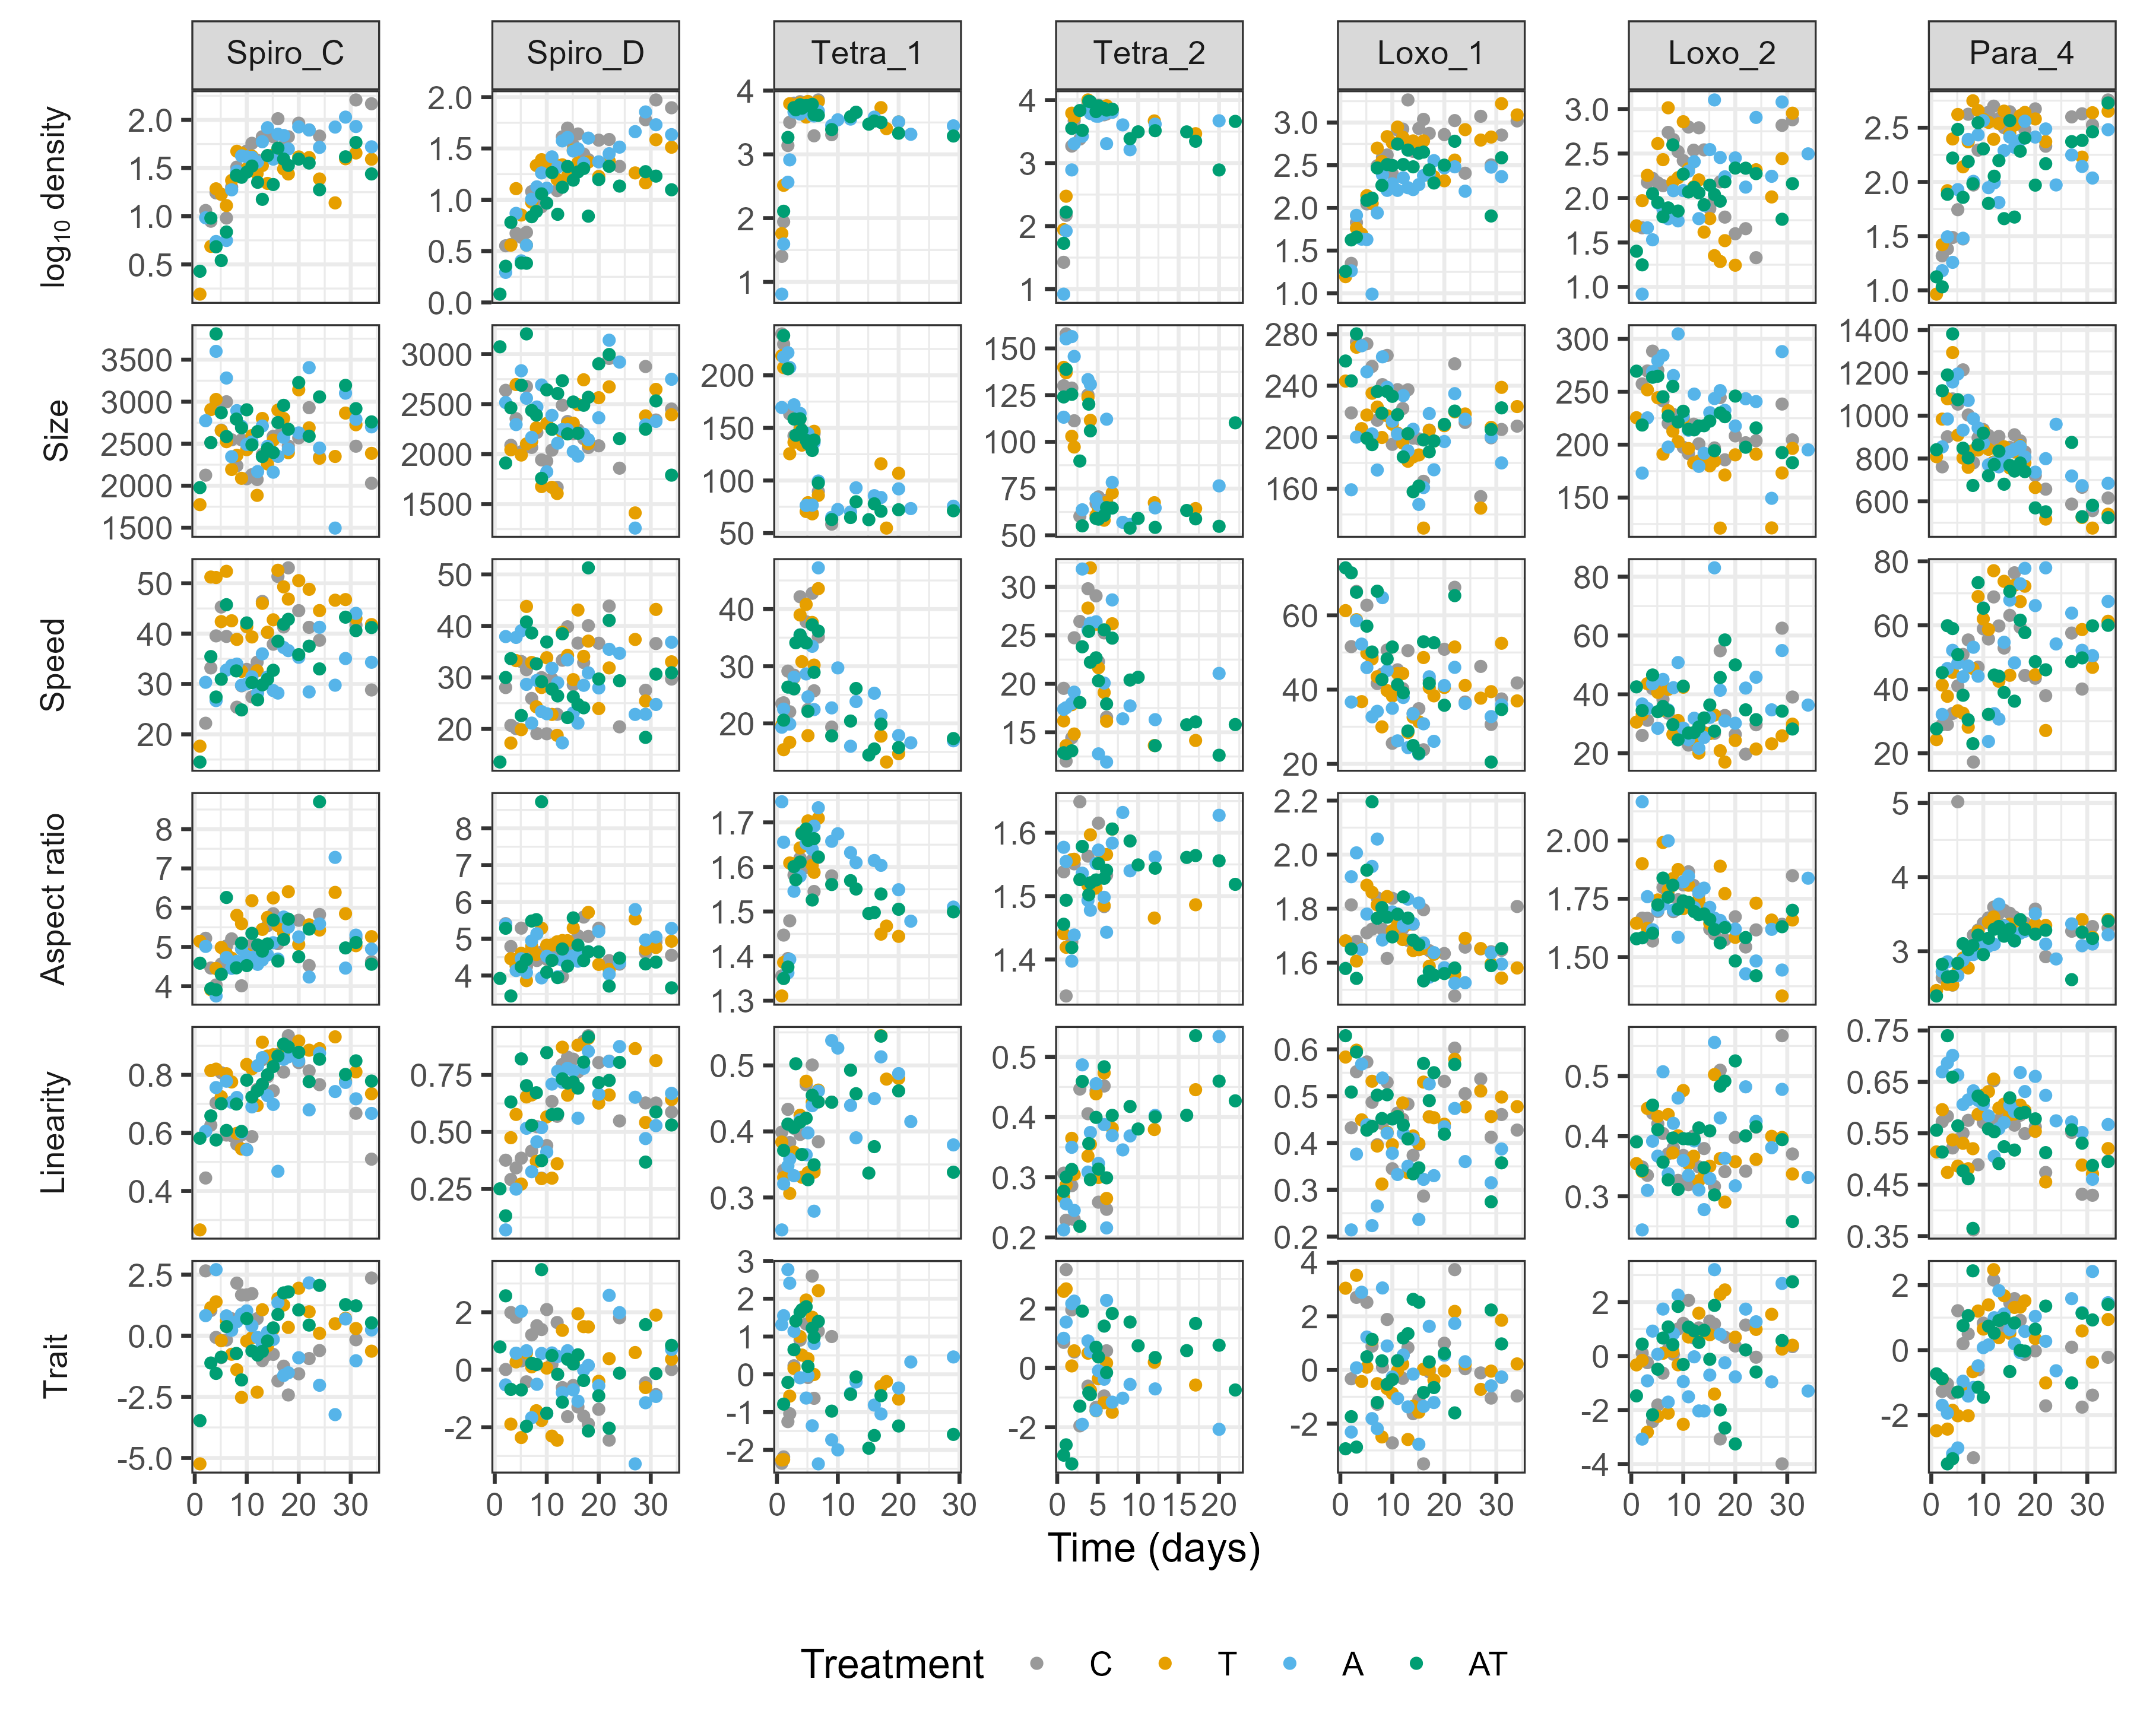
\includegraphics[width=6in,height=\textheight]{figures/cilia_pop-traits-time.png}

}

\caption{\label{fig-cilia-pop-traits-time}Log-transformed populations
and trait changes over time for the ciliate system. The traits show the
mean values in the sampled population at each time point. Size indicates
the top-down area of the cell in \textmu\(\mathrm{m}^{2}\). Speed
indicates the average movement speed in \textmu\(\mathrm{m \, s}^{-1}\).
Aspect ratio is the ratio of the longest cell dimension relative to the
shortest. Linearity indicates the cell movement linearity i.e.~a value
of 1 is perfectly linear while a value of 0 is Brownian motion. Trait
indicates the aggregate trait - the first axis of a PCA fitted across
the four measured traits for each strain and treatment combination.}

\end{figure}%

The cyanobacteria populations grew logistically in the control and
temperature treatments, but maintained stable or slightly-decreased
populations in the atrazine and atrazine-temperature treatments
(Figure~\ref{fig-cyano-pop-traits-time}).

\begin{figure}

\centering{

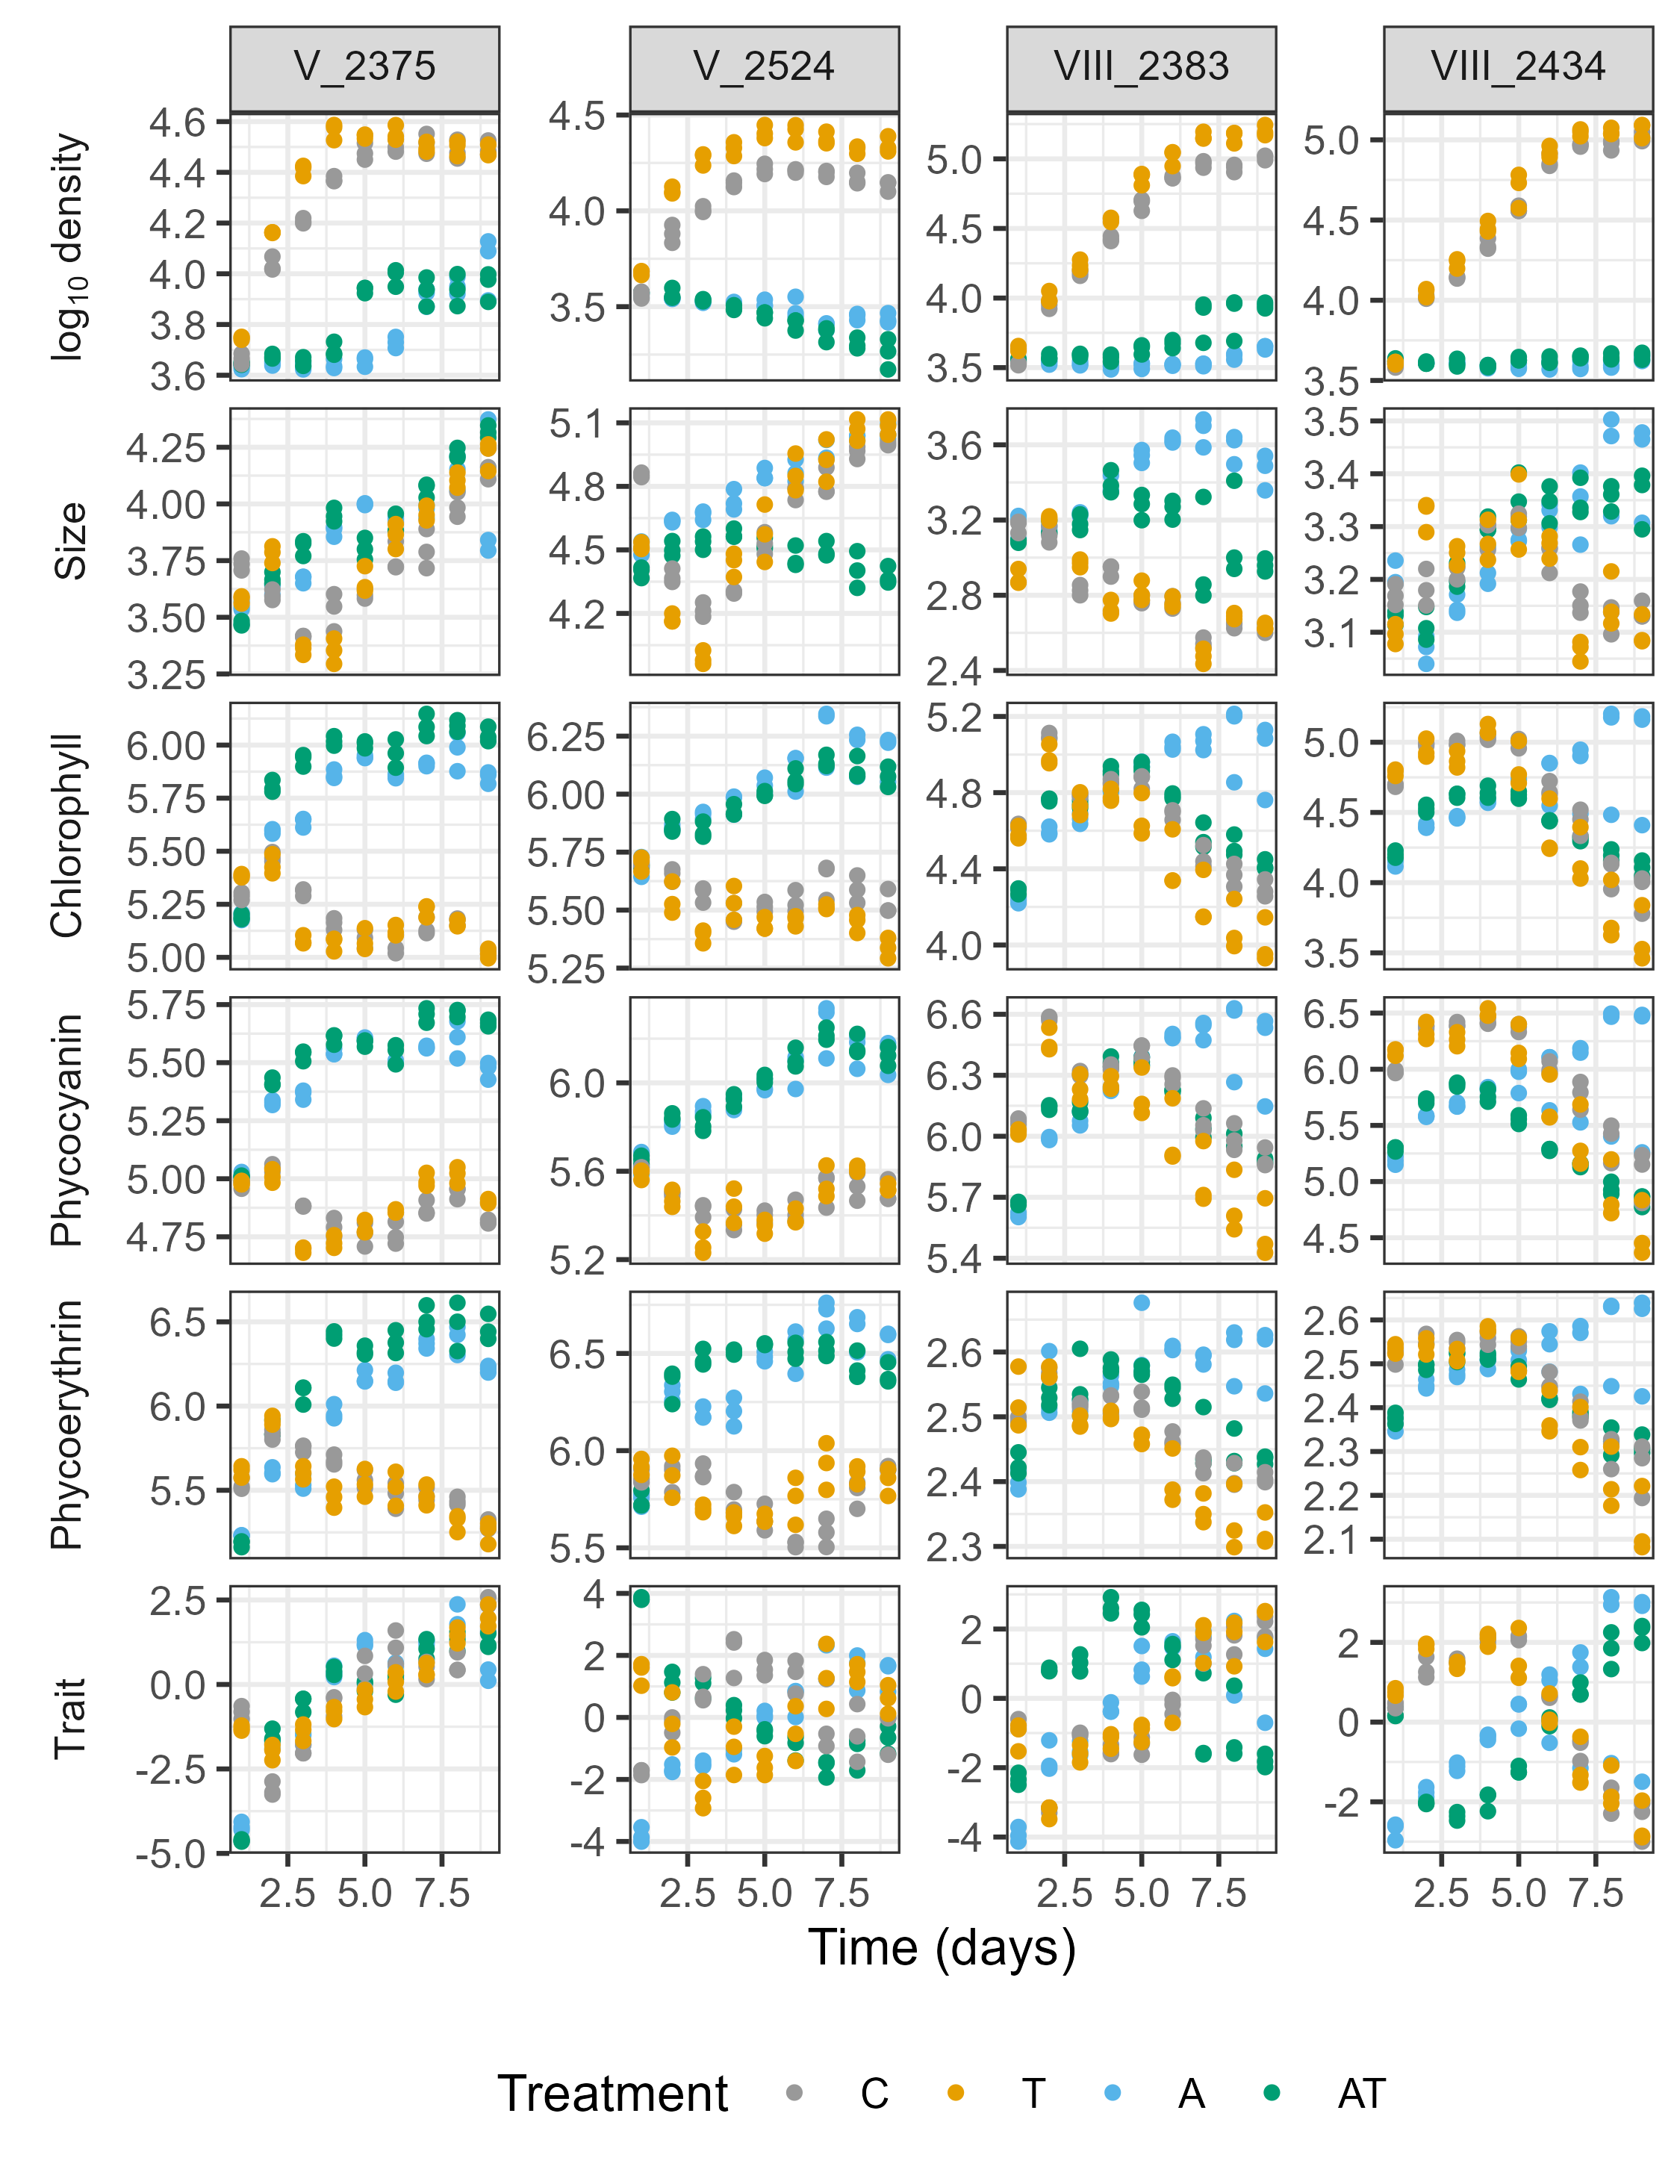
\includegraphics[width=5in,height=\textheight]{figures/cyano_pop-traits-time.png}

}

\caption{\label{fig-cyano-pop-traits-time}Log-transformed populations
and trait changes over time for the ciliate system. The traits show the
mean values in the sampled population at each time point. Measured
traits (size, chlorophyll, phycocyanin, and phycoerythrin) are expressed
in arbitrary units. Size is proportional to the cell diameter, and the
three pigment channels are defined by their excitation and fluorescence
(see supporting information). Trait indicates the aggregate trait - the
first axis of a PCA fitted across the four measured traits for each
strain and treatment combination.}

\end{figure}%

Individual traits (and therefore the aggregate trait) changed
substantially throughout the experiment for both the ciliate and
cyanobacteria systems (Figure~\ref{fig-cilia-pop-traits-time},
Figure~\ref{fig-cyano-pop-traits-time}). These aggregate traits also
contained the majority of the trait variation, and well-summarised the
four functional traits of each study system into a single variable
(Figure~\ref{fig-PC-var-explained}, Figure~\ref{fig-PC-var-explained})

\begin{figure}

\centering{

\includegraphics{figures/PC_var_explained.pdf}

}

\caption{\label{fig-PC-var-explained}The amount of variance explained by
the first component of the PCA for the ciliate and cyanobacteria
systems. These values indicate how much information is kept when the
traits are combined into a single aggregate trait. The horizontal dashed
line indicates the mean explained variance across all strains and
treatments (\(53.6\%\)).}

\end{figure}%

Populations of both systems exhibited mostly nonzero intrinsic growth
and negative density-dependence (Figure~\ref{fig-cilia-td-general},
Figure~\ref{fig-cyano-td-general}). Intrinsic growth rates of
\emph{Tetrahymena} strains were consistently higher than that of the
other strains and \emph{Spirostomum} strains exhibited stronger negative
density-dependence (i.e.~stronger self-limitation). Environmental
conditions had moderate and variable effects on how ciliate populations
grew. In the cyanobacteria system, intrinsic growth and
density-dependence were comparable across strains
(Figure~\ref{fig-cyano-pcgr}). However, environmental conditions had
greater effects on these parameters; the addition of atrazine
substantially reduced intrinsic growth rates (to the point of being
negative in cases).

The traits of both systems exhibited generally negative trait-dependence
(Figure~\ref{fig-cilia-td-general}, Figure~\ref{fig-cyano-td-general}).
In the ciliate system, intrinsic trait change
(Figure~\ref{fig-cilia-dT}) was generally not significantly different
from zero, but estimates varied across environmental conditions in
\emph{Tetrahymena} strains. The trait-dependence of trait change in
ciliates was also strongest for these strains. In the cyanobacteria
system, intrinsic trait change was often significantly different from
zero and mostly positive (Figure~\ref{fig-growth-dtrait}).

\section{Population density and population
change}\label{population-density-and-population-change}

\subsection{Ciliate}\label{ciliate-1}

\begin{figure}

\centering{

\includegraphics[width=4in,height=\textheight]{figures/cilia_pcgr.pdf}

}

\caption{\label{fig-cilia-pcgr}Density-dependence of ciliate per-capita
growth rate in the different treatments.}

\end{figure}%

\subsection{Cyanobacteria}\label{cyanobacteria-1}

\begin{figure}

\centering{

\includegraphics[width=4in,height=\textheight]{figures/cyano_pcgr.pdf}

}

\caption{\label{fig-cyano-pcgr}As Figure~\ref{fig-cilia-pcgr} but for
the cyanobacteria system}

\end{figure}%

\section{Trait values and trait
change}\label{trait-values-and-trait-change}

\subsection{Ciliate}\label{ciliate-2}

\begin{figure}

\centering{

\includegraphics[width=4in,height=\textheight]{figures/cilia_dT.pdf}

}

\caption{\label{fig-cilia-dT}Trait-dependence of ciliate trait change in
the different treatments.}

\end{figure}%

\subsection{Cyanobacteria}\label{cyanobacteria-2}

\begin{figure}

\centering{

\includegraphics[width=4in,height=\textheight]{figures/cyano_dT.pdf}

}

\caption{\label{fig-cyano-dT}As Figure~\ref{fig-cilia-dT} but the
cyanobacteria system.}

\end{figure}%

\section{Fitted regression
coefficients}\label{fitted-regression-coefficients}

\subsection{Ciliate}\label{ciliate-3}

\begin{figure}

\centering{

\includegraphics[width=4in,height=\textheight]{figures/cilia_td_general.pdf}

}

\caption{\label{fig-cilia-td-general}Fitted model parameters showing
intrinsic population/trait change (left), density-dependence (centre),
and trait dependence (right) in seven strains of ciliates. Large rows
indicate whether growth or trait change is being examined and subrows
indicate whether the coefficients are from the single-variable or
augmented model. Points indicate the mean, error bars indicate the 95\%
confidence intervals, and asterisks indicate parameters are
significantly different from zero (vertical black line).}

\end{figure}%

\subsection{Cyanobacteria}\label{cyanobacteria-3}

\begin{figure}

\centering{

\includegraphics[width=4in,height=\textheight]{figures/cyano_td_general.pdf}

}

\caption{\label{fig-cyano-td-general}As
Figure~\ref{fig-cilia-td-general}, but for four strains of the
cyanobacteria genus \emph{Synechococcus}.}

\end{figure}%

\section{Model goodness-of-fit}\label{model-goodness-of-fit}

\subsection{Ciliate}\label{ciliate-4}

\begin{figure}

\centering{

\includegraphics{figures/R2.pdf}

}

\caption{\label{fig-R2}The coefficient of determination i.e., r-squared,
for the cilia and cyanobacteria system models. The mean values across
strains and treatments are shown by the horizontal dashed lines.}

\end{figure}%

In the ciliate system, the \(R^2\) of the model fit was generally below
0.5 for both growth and trait changes for all treatments and was
generally unaffected by whether the single- or both-predictor model was
used (Figure~\ref{fig-R2}). \emph{Tetrahymena} strains were generally
better-fitting but still without substantial model support. In the
cyanobacteria system, the treatments without atrazine were substantially
better-fitting than those with atrazine added (Figure~\ref{fig-R2}).
Additionally, while the goodness-of-fit of the growth predictions were
only marginally improved by the addition of the full model, the trait
change predictions were greatly improved by including the full model.



\end{document}
